%!TEX root = thesis.tex

\chapter{Pick and place}
\label{chap:pick_place}

The implementation of a benchmark pick and place task which is executable on a simulator as well as on the real robot states one of the objectives of this project. The task consists of various stages which have to be planned using the planning framework introduced in the previous chapter. The overview at the beginning of this chapter provides information about general grasping tasks, explains the process step by step and describes the successive stages that have to be executed. The second part focuses on how pick and place tasks are planned and executed using the motion planning framework that was described in the previous chapter. The third section explains the implementation of the benchmark pick and place task in detail and describes the involved message types and action servers. The last section discusses some observations that have been made during the implementation process.

\section{Overview}

A pick and place task is the process of grasping an object, lifting it and dropping it at a target position. Humans can do that without even thinking about it. But directing a robot to perform a pick and place task reveals how difficult and complex it is and how much planning has to be involved to achieve the desired result. A planner would possibly require exact knowledge about the robot and it's environment, including the objects to grasp and the obstacles around. Collisions that could harm the robot have to be avoided but other collisions are necessary when the robot has to get in contact with the world. The gripper definitely collides with the object to pick, but only during grasping and holding. Therefore there has to be a mechanism to explicitly tell the planner that specific collisions are allowed during particular stages of the operation. Moreover, after grasping an object it has to be considered as an additional part of the robot. That means for the planning domain, that the grasped object should be included to the definition of the robot during subsequent planning requests because it possibly increases the size of the end effector that carries the object. \\

Stationary objects usually stand or lie on a surface, called the \emph{support surface}. During the interaction with an object, possible collisions with the support surface have to be taken into account. It is also possible that the whole process underlies additional constraints, so called \emph{path constraints}. This type of constraint has to be enforced along the whole path which the grasped object takes during the operation. For example, when carrying a glass filled with liquid it has to remain in an upright position, otherwise the liquid is lost. That means, the glass has to be held in a specific orientation during the whole task. This can be described as an so-called \emph{orientation constraint} which is a special type of a path constraint. The planning solution has to provide mechanisms to define and enforce such types of \emph{path constraints}. \\

\begin{figure}[ht]
	\centering
  	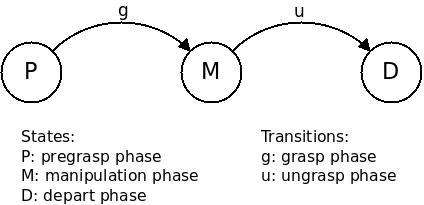
\includegraphics[width=0.5\textwidth]{images/state_trans.jpg}
	\caption{State transition diagramm for a pick and place task}
	{\scriptsize Image inspired by \citep{kang1994}}
	\label{fig:state_trans}
\end{figure}

\citep{kang1994} propose a method for \emph{temporal segmentation} of arbitrary grasping tasks. They divide each task into sequences of \emph{subtasks} that \emph{can be represented as series of states and transitions}. According to their notion, a pick and place operation is divided into 5 phases.

\begin{itemize}

\item \textbf{Pregrasp phase} \\

This phase starts at an arbitrary robot configuration. The hand is moved towards the grasp location and the fingers have to be adjusted to preshape the gripper in a way that allows to enclose the object to grasp (or at least that part that is used to clutch it). The required gripper configuration depends on the size and shape of the object to grasp and the structure of the gripper.

\item \textbf{Grasp phase} \\

This is the stage where the robot gets in contact with the object. The gripper closes around the object and applies as much force as necessary to be able to take and hold it. The grasp phase states the transition between the \emph{pregrasp} and the \emph{manipulation} phase.

\item \textbf{Manipulation phase} \\

The grasped object is enclosed by the gripper and considered to be part of the robot configuration. 
During \emph{manipulation} phase, the object is translated towards the place location. Possible path constraints have to be enforced whilst that stage.

\item \textbf{Ungrasp phase} \\

The manipulator reached at the goal location and the gripper opens and releases the object. This is the transition between \emph{manipulation} and \emph{depart} phase.

\item \textbf{Depart phase} \\

The object was placed at the target location and relased by the gripper. Now the manipulator retreats from the object. After that the entire task is completed.

\end{itemize}

The corresponding state transition diagram can be seen in Figure\ref{fig:state_trans}. The task is only considered to be complete if each single stage was successfully executed. Necessary planning parameters like the grasp location and gripper configurations are usually provided by a grasp planner. This is an additional node within the planning pipeline that can be used to identify objects in the environment of the robot, usually based on 3D sensor data and calculate the corresponding grasp parameters. Explaining the functionality of grasp planners is beyond the scope of this project though the section about implementing the reference task discusses the used parameters in greater detail and shows what data would usually be delivered by the grasp planner. \\

\section{Pick and place tasks in MoveIt}

\begin{figure}[ht]
	\centering
  	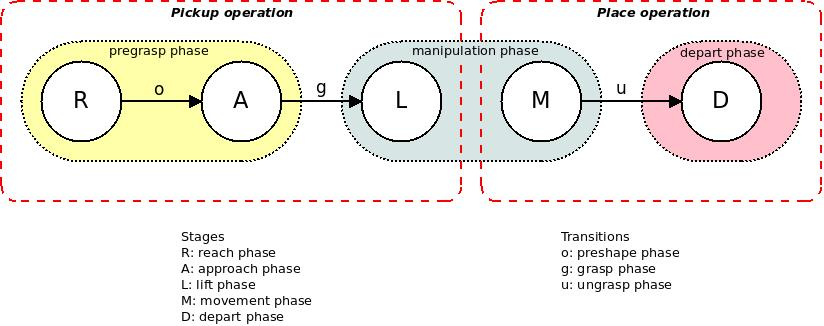
\includegraphics[width=1.0\textwidth]{images/pick_place_states.jpg}
	\caption{Extended state transition diagram}
	\label{fig:pick_place_states}
\end{figure}

The robot motions during the phases described in the previous section need to be planned. Each single stage requires to plan trajectories that are free of accidental collisions, respect the limits of the robot and enforce possible additional constraints. The task can only be considered executable if a valid motion plan for each single stage exists. Planning pick and place tasks in MoveIt requires to split them into two distinct operations, namely the \emph{pickup} operation and the \emph{place} operation. The explanation of those operations requires to further subdivide the phases described in the previous section. Figure \ref{fig:pick_place_states} shows the resulting state transition diagram.\\

The pickup operation starts at an arbitrary robot configuration. In the \emph{reach} stage, the manipulator has to be brought into a position close to the object to grasp, but in a distance which allows the gripper to open safely without touching the object. The \emph{preshape} stage sets the gripper into the \emph{pregrasp posture} which means the fingers are brought into a shape that allows to completely enclose the object (or at least that part that is used to clutch it). During the \emph{approach} phase the gripper moves towards the final grasp pose along the defined approach direction. The \emph{grasp} phase moves the gripper fingers into the \emph{grasp posture} - a configuration that encloses the object and applies as much force as necessary to be able to take and hold it. The resulting collisions between the gripper links and the object have to be ignored by the planner. From that point on the grasped object is \emph{attached} to the gripper, which means it is considered to be an additional part of the end effector during subsequent planning steps. The pickup operation completes lifting the object along the retreat direction (\emph{lift} phase). Figure \ref{fig:pickup} shows the stages of the pickup phase.

\begin{figure}[h]
	\centering
  	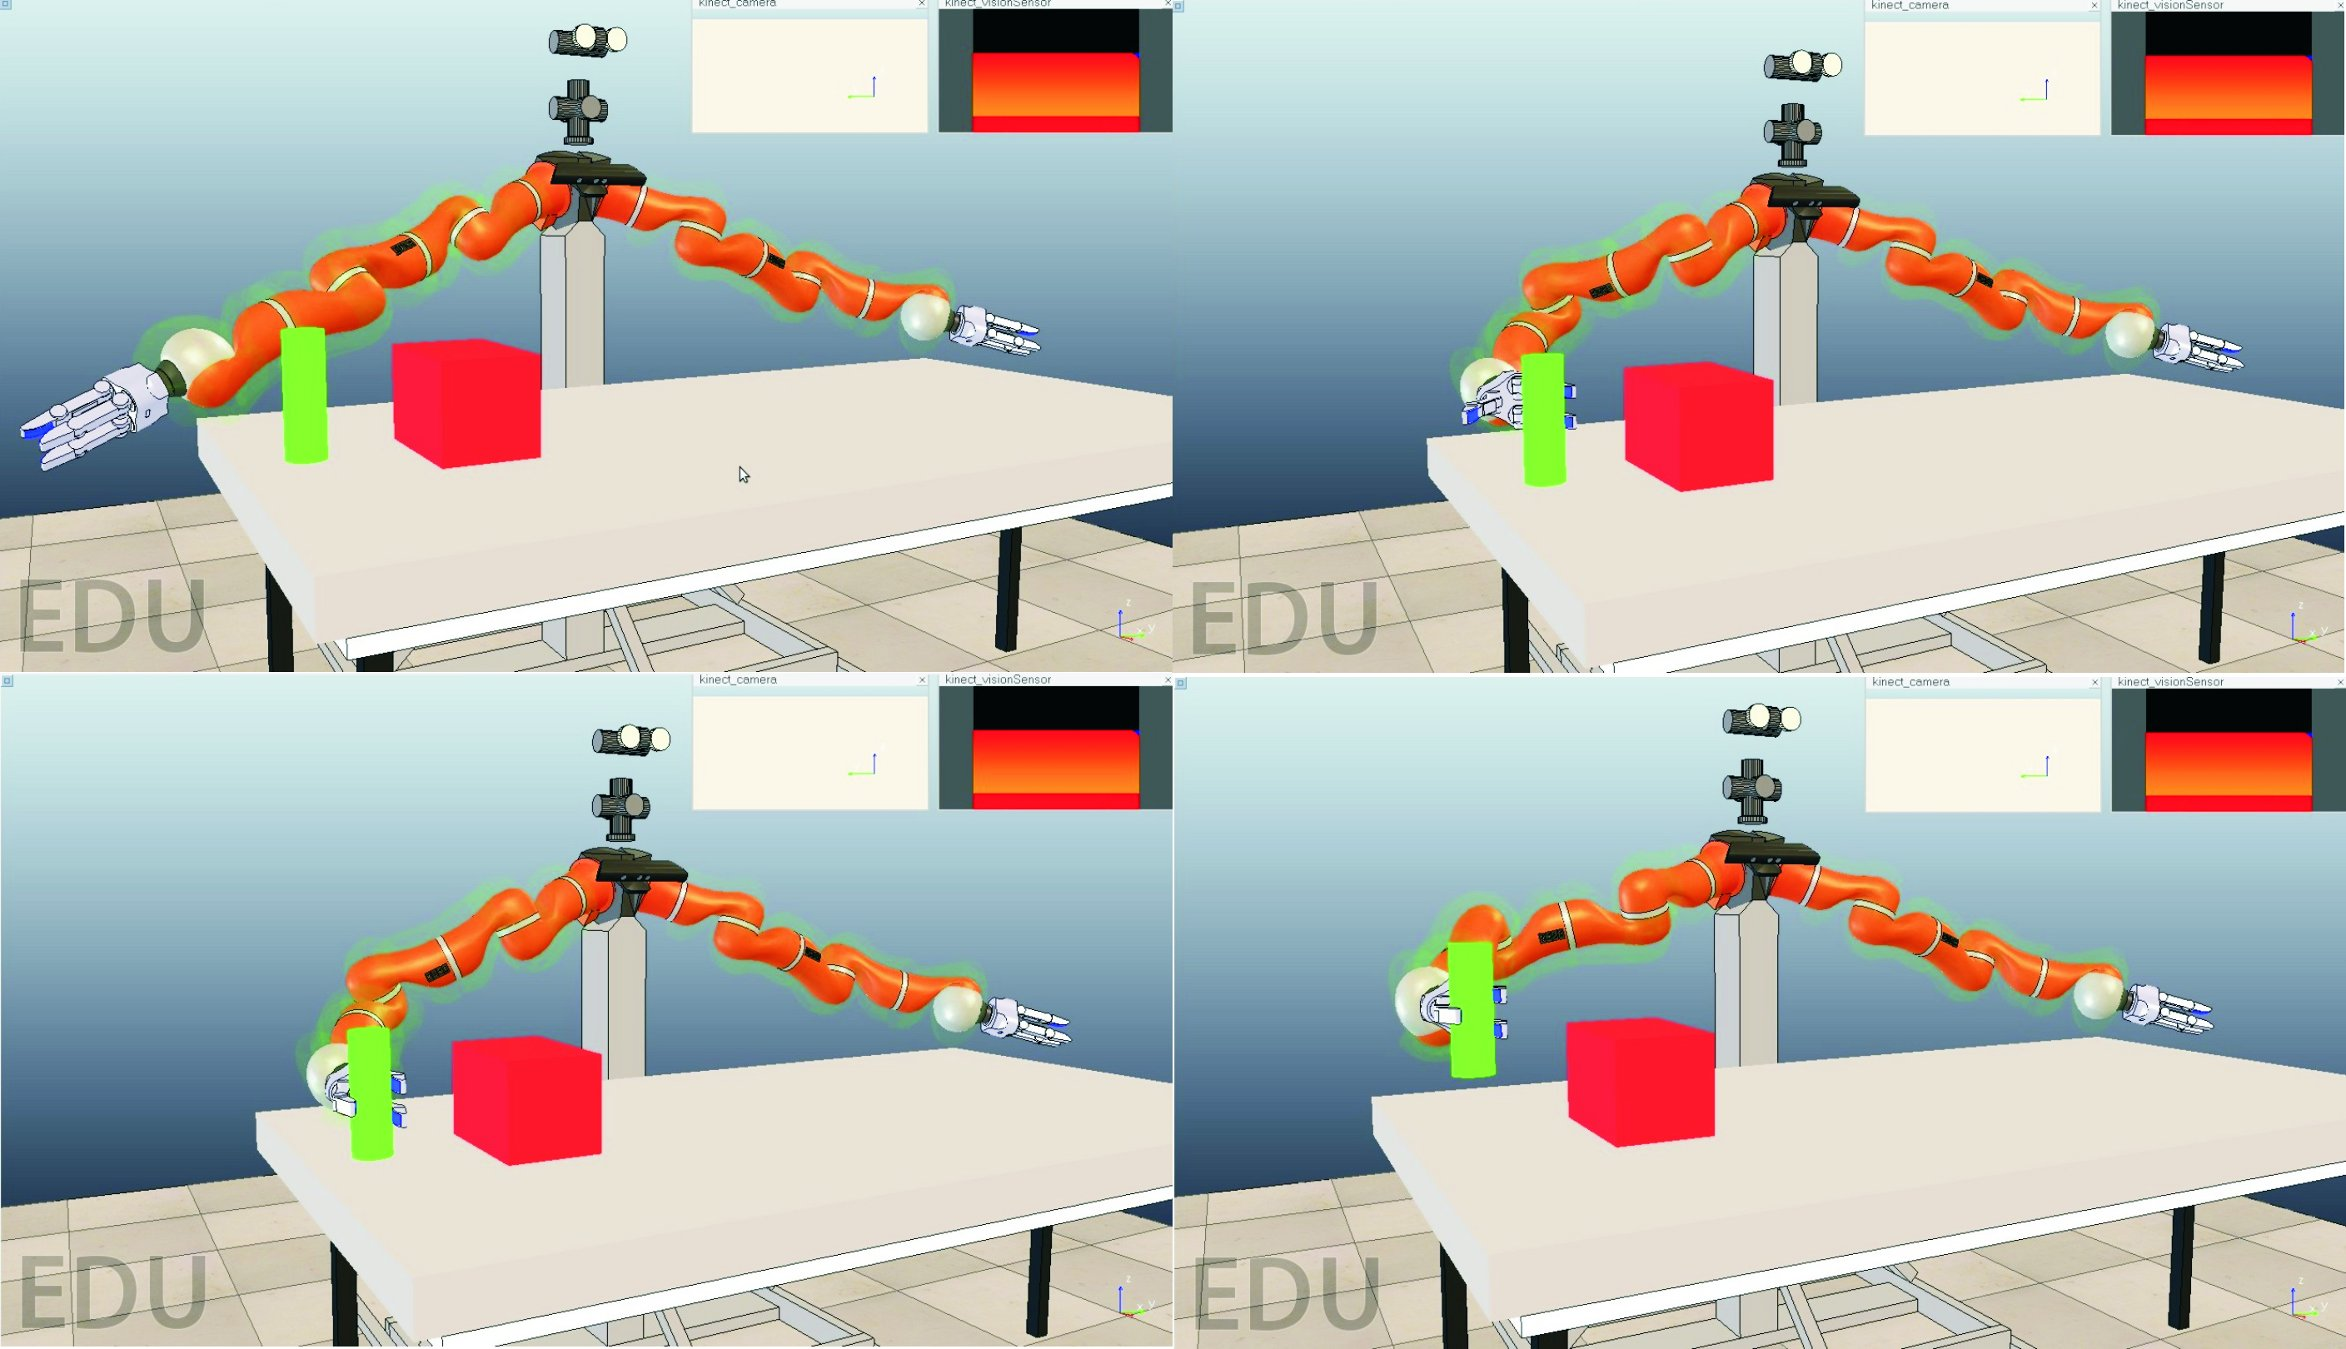
\includegraphics[width=0.75\textwidth]{images/pickup.jpg}
	\caption{Stages of the pickup phase in the simulator}
	\label{fig:pickup}
\end{figure}

The place operation starts after a successful pickup. The grasped object is enclosed by the gripper and it is considered to be part of the robot. During the \emph{movement} phase, the object is translated towards the final \emph{place location}. The planner has to take into account that the object could possibly get into contact with the support surface again when it's final position is reached. At that stage, the gripper opens (\emph{ungrasp} phase) and releases the object. Now the object has to be treated as an obstacle again and the planner is forced to avoid collisions with it. The place operation completes after the manipulator has moved away from the object (\emph{depart} phase) along the specified retreat direction. The stages of the placement phase can be seen in Figure \ref{fig:placement}.

\begin{figure}[h]
	\centering
  	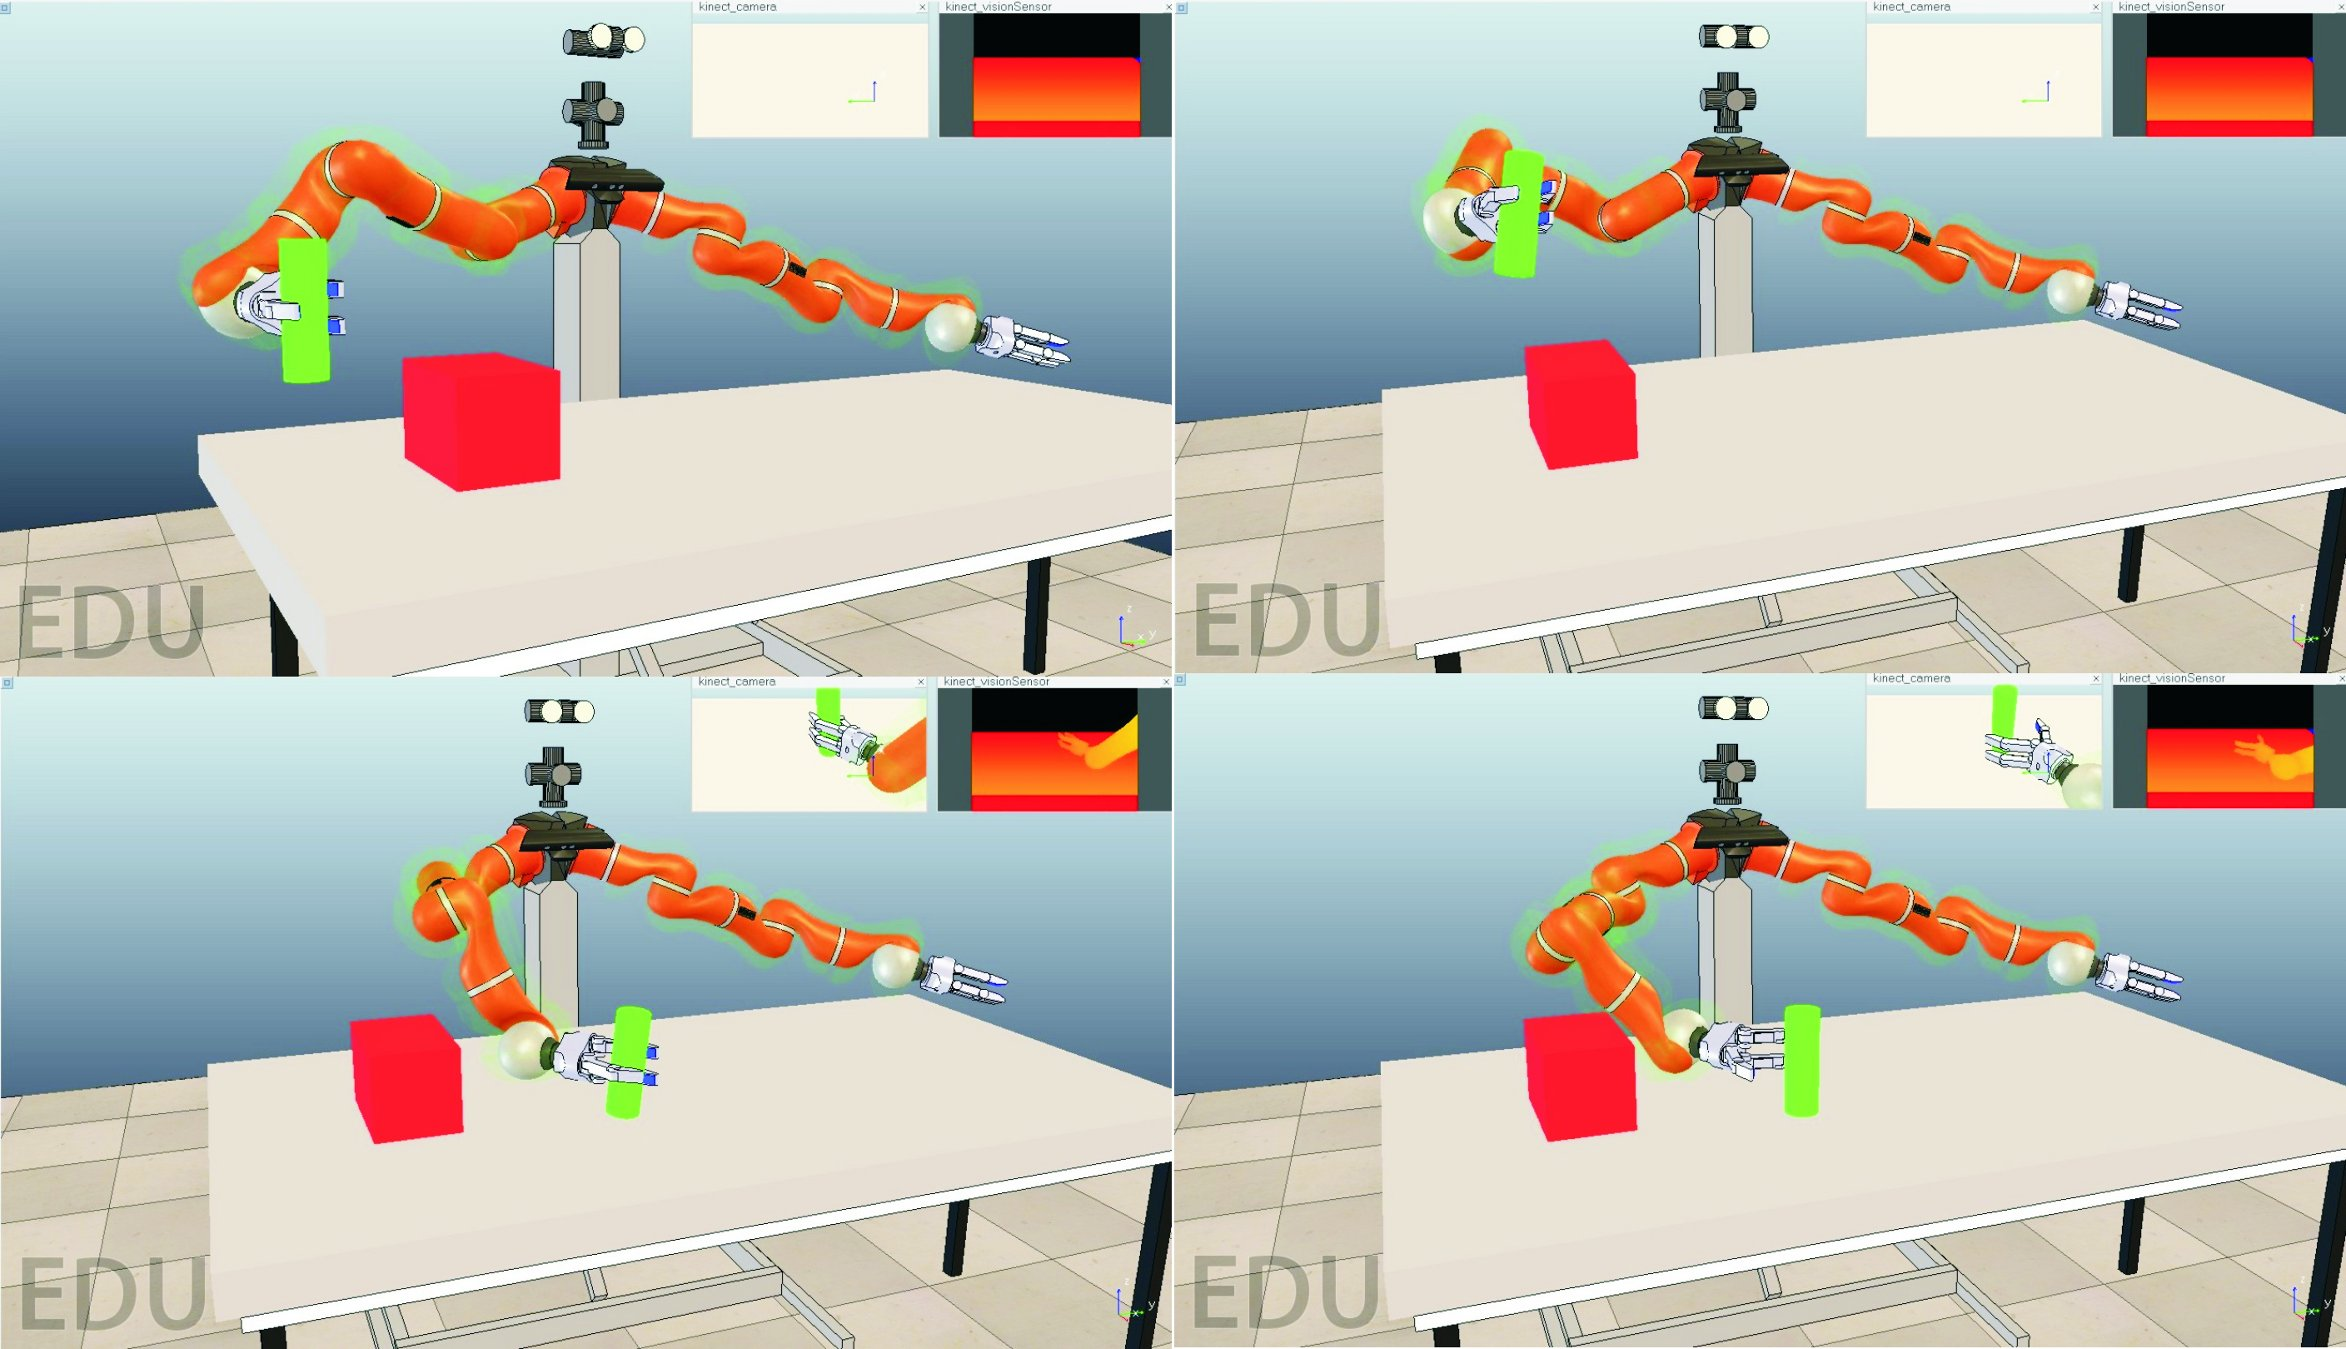
\includegraphics[width=0.75\textwidth]{images/placement.jpg}
	\caption{Stages of the placement phase in the simulator}
	\label{fig:placement}
\end{figure}

%The explanation of those operations requires to further subdivide the phases, described in the previous section. This results in the state transition diagram that can be seen in Figure \ref{fig:pick_place_states}. The pregrasp phase is split into \emph{reach}, hand \emph{preshape} and \emph{approach} phase. During the reach phase, the manipulator is moved into a position close to the object to grasp, but in a distance that allows the gripper to open safely without touching the object. This position is called the \emph{pre-grasp pose}. The approach phase brings the opened gripper towards the final \emph{grasp pose}. 
%The preshape phase is the transition between the reach and the approach phase. During that stage the gripper needs to  bring it's fingers into a configuration that allows to enclose the object. This configuration is called the \emph{pre-grasp posture}. The manipulation phase is divided into two phases, namely the lift phase and the movement phase. There is no transition between those two stages because the pickup operation completes after the lift phase and the place operation starts at the movement phase. Planning of those operations happens by using the corresponding action servers that are advertised by the \path{move_group} node.\\

%The structure of the request messages and the involved parameters are described in the next section. The result of a successful request is a motion plan that contains trajectories for all stages of the planned operation.

The planning of the described operations make use of action servers which are advertised by the \path{move_group} node, namely the \emph{pickup action server} and the \emph{place action server}. The pickup and placement requests are composed from a large number of parameters that are explained in detail in the next section. Objects contained in the task environment have to be added to the MoveIt planning scene. This can be done manually by publishing them to corresponding topics or by a MoveIt configuration to monitor the environment through sensor data, e.g. from a Kinect camera. For the sake of simplicity, all involved objects were manually added in the benchmark task. Pickup- and place action servers provide the ability to choose whether to execute motion plans immediately or to just perform the planning part and return the resulting trajectories for later execution. Immediate execution is often preferable because MoveIt executes the trajectories and handles additional requirements like attaching and detaching the grasped object in time. It has the drawback, however, that occasionally overly long and unnatural trajectories are executed immediately because they might be formally valid solutions for the given planning problem, though they are unsuitable for a human observer. Therefore a safety mechanism which can interrupt an execution in face of problems needs to be added. The second, planning-only method allows to visualize the resulting trajectories and then decide whether to execute them or not. But then each single trajectory stage has to be executed manually which also includes attaching or detaching objects to the manipulator. The advantage of this method is the clean separation between planning and execution, allowing maximum control over the execution flow. Therefore this method was favoured during benchmark task implementation.

\section{Implementation of the benchmark task}

This section describes the implementation of the benchmark pick and place task in detail. The source code can be found in the \path{uibk_moveit_tests} package. The workspace is the table in front of the robot covered with a 9 cm thick foam mat. This mat will be declared as the support surface later on. The object to grasp is a cylinder with 4 cm radius and a height of 25 cm. The cylinder is located on a fixed, known position. A cube with an edge length of 20 cm acts as additional obstacle within the workspace. The goal of the task is to pick the cylinder up, using the right arm of the robot and place it at the goal location without colliding with the obstacle or other parts within the robot's environment. The implementation makes use of the previously described pick and place functionality. The necessary steps are explained in the following subsections.

\subsection{Creating the environment}
\begin{figure}[h]
	\centering
  	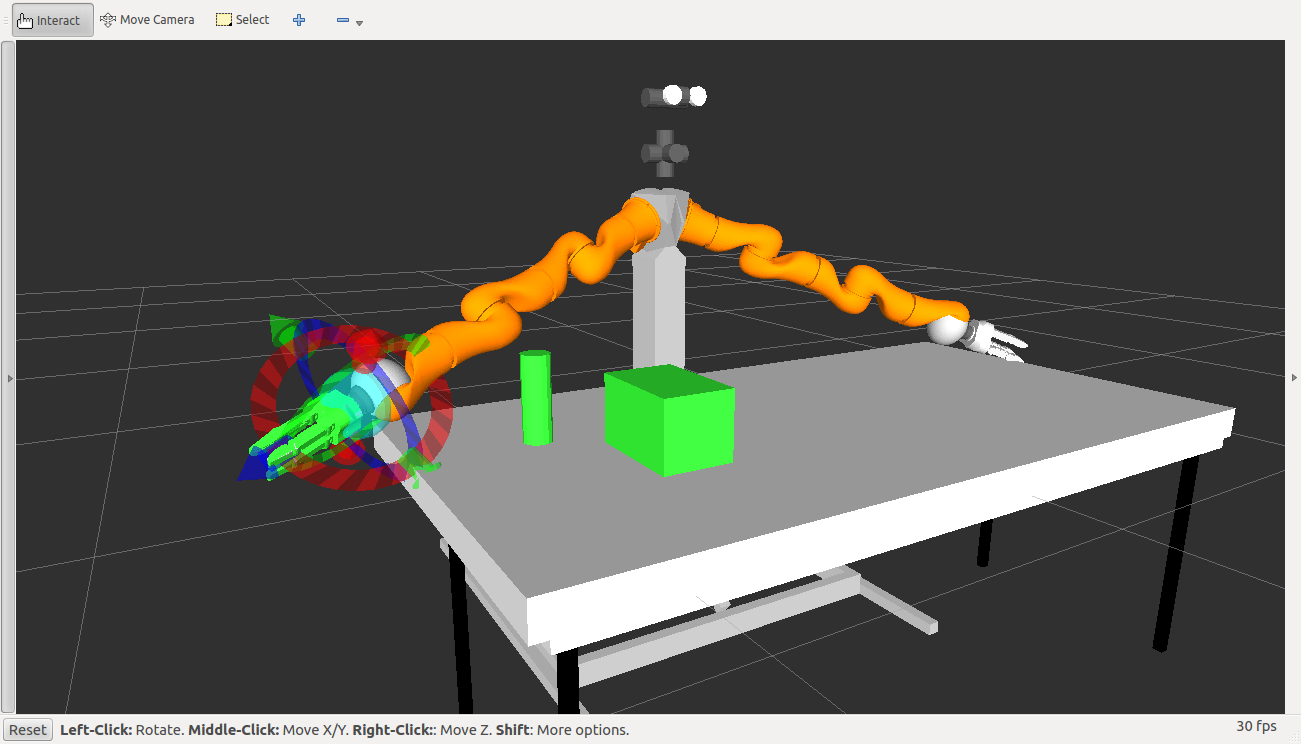
\includegraphics[width=0.75\textwidth]{images/task_env.png}
	\caption{Planning scene after inserting the collision objects}
	\label{fig:task_env}
\end{figure}
As MoveIt is currently not configured to use sensor data, it has to be informed about the task environment. The table and the surface mat (\path{table_surface_link}) are already part of the URDF description but the cylinder and the obstacle have to be added to the planning scene. This is done utilizing the \emph{PlanningSceneInterface} class that provides functionality to manipulate the current planning scene. The \emph{CollisionObject} type is used to describe those objects. Both of them are primitive shapes. Necessary parameters are the shape type, dimensions and pose. Additionally each \emph{CollisionObject} needs a unique ID which is used to identify the shape within the planning scene. Listing \ref{lst:obstacle} shows the necessary code for creating the obstacle, Figure \ref{fig:task_env} shows a visualization of the task environment after adding the \emph{CollisionObjects}.

\lstset{style=customc}
\begin{minipage}{\linewidth}
\begin{lstlisting}[caption={Creating the obstacle}, label=lst:obstacle]
std::vector<moveit_msgs::CollisionObject> collision_objects;
// create an obstacle
shape_msgs::SolidPrimitive box;
box.type = box.BOX;
box.dimensions.resize(3);
box.dimensions[0] = 0.2;
box.dimensions[1] = 0.2;
box.dimensions[2] = 0.2;

/* A pose for the box (specified relative to frame_id) */
geometry_msgs::Pose box_pose;
box_pose.orientation.w = 1.0;
box_pose.position.x = 0.15;
box_pose.position.y = 0.10;
box_pose.position.z = 0.1 + SUPPORT_SURFACE_HEIGHT;

obstacle.primitives.push_back(box);
obstacle.primitive_poses.push_back(box_pose);
obstacle.operation = obstacle.ADD;

collision_objects.push_back(obstacle);
// Now, let's add the collision object into the world
planning_scene_interface_->addCollisionObjects(collision_objects);
\end{lstlisting}
\end{minipage}

\subsection{Generating possible grasps}

\begin{figure}[h]
	\centering
  	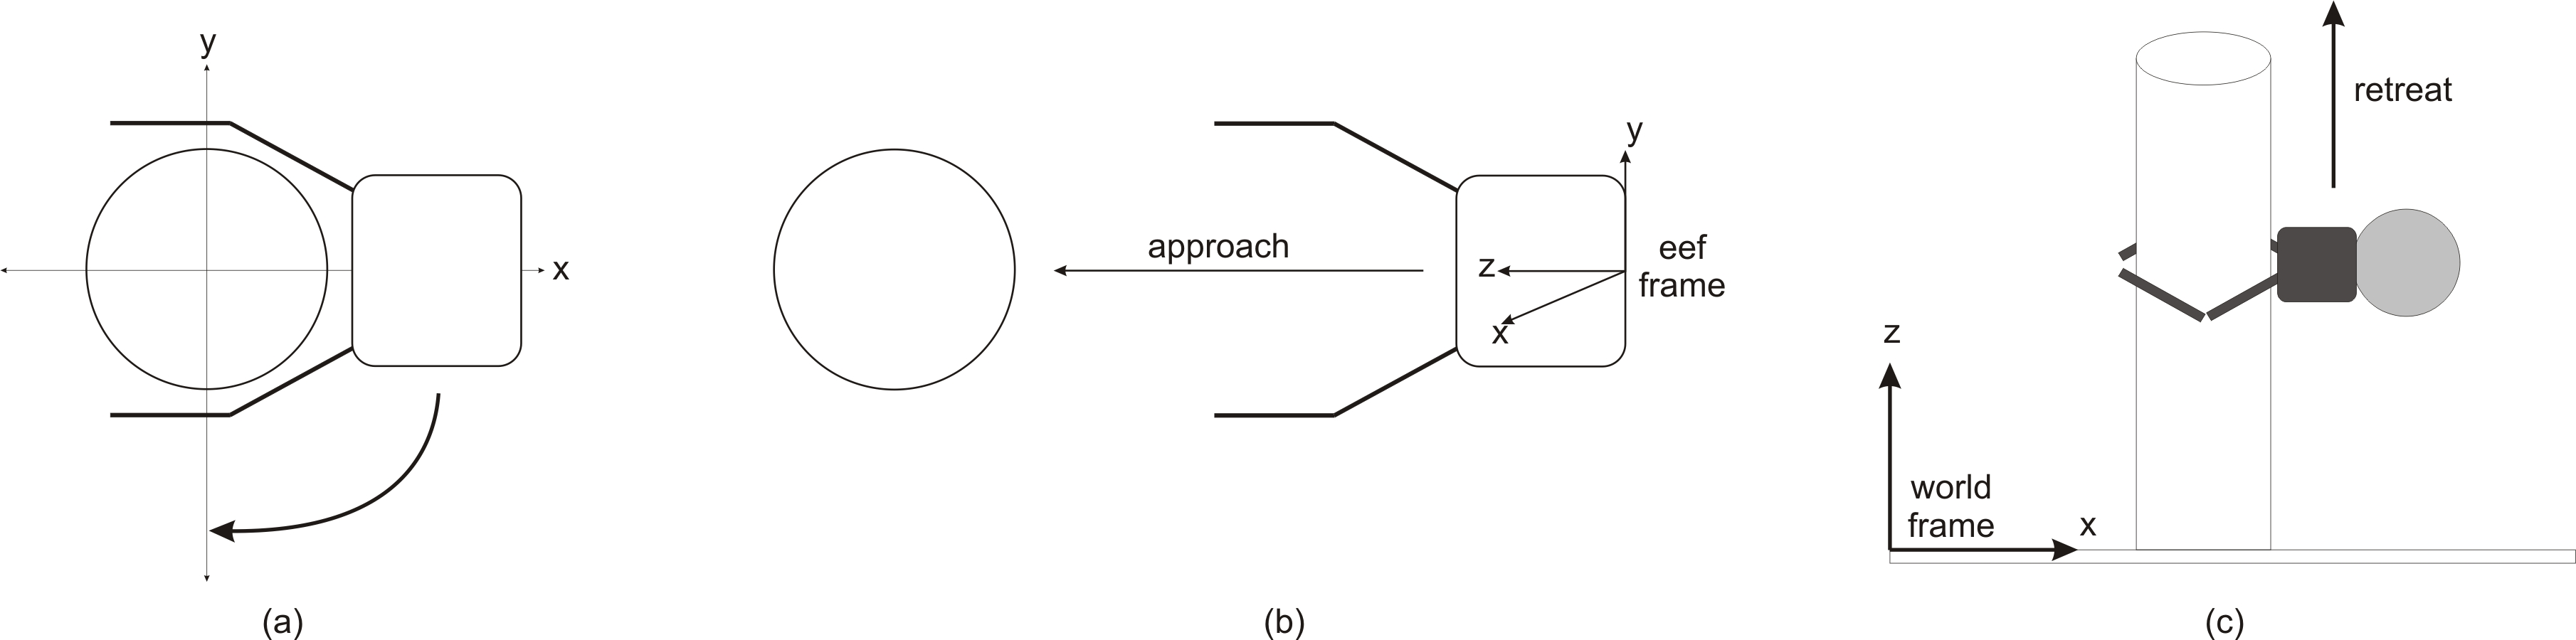
\includegraphics[width=1.0\textwidth]{images/grasp_a-c.jpg}
	\caption{Grasp poses, gripper approach and retreat}
	\label{fig:grasp_stages}
\end{figure}

Picking up an object can always be done in several ways. Depending on the shape of the object there always multiple alternatives how gripper can safely approach and grasp. Providing a number of different grasps raises the probability that the pickup request will be successful. Before calling the pickup action server it is necessary to generate a set of possible grasps for the object to pick. This information is usually provided by a grasp planner. The sample task encapsulates the grasp planner functionality within the \path{generateGrasps()} method. This method takes the current pose of the cylinder as input and calculates 10 possible grasp poses along an imaginary circle segment around the cylinder location (Figure \ref{fig:grasp_stages}a). Grasps are defined in terms of the \emph{Grasp} data structure. The following paragraphs describe the involved parameters and how they were determined in the benchmark task implementation.

\paragraph{Grasp ID} A string that uniquely identifies the grasp. As usually many different grasps are provided for each pickup request, this ID can be used to identify the grasp which is finally picked to solve the planning problem. The grasp IDs are formed according to the pattern \texttt{[Grasp]x}, where $x \in [0,10]$ 

\paragraph{Pre-grasp/grasp posture} Describes the shape of the hand before/after grasping the object.
Pre-grasp and grasp postures are joint trajectories for the gripper, containing just one trajectory point stating the target configuration for the gripper in the opened respectively the closed state.

\paragraph{Pre-grasp approach and post-grasp retreat} The pre-grasp approach and the post-grasp retreat are defined as \emph{GripperTranslation}, as can be seen in Listing \ref{lst:translation}. This is a special message type that describes the direct gripper movement from one position towards a target. The direction is defined as a three dimensional vector. The length of the translation can be set in a flexible way by specifying a desired distance and a minimum distance. That means that the location where the gripper needs to open is not explicitly set and can be any point along the approach vector between minimum distance and desired distance. Experiments showed that the success rate is higher if the grasp parameters allow some flexibility to the planner at certain points. The approach vector depends on the grasp pose and points along the z-axis of the end effector frame towards the object (Figure \ref{fig:grasp_stages}b). The gripper retreat vector points up, along the z-axis of the world (Figure \ref{fig:grasp_stages}c).

\lstset{style=customc}
\begin{minipage}{\linewidth}
\begin{lstlisting}[caption={Definition of gripper translations}, label=lst:translation]
// gripper approach
GripperTranslation gripper_approach;
gripper_approach.desired_distance = 0.2; // cm
gripper_approach.min_distance = 0.1; // cm
gripper_approach.direction.header.frame_id = EE_PARENT_LINK;
gripper_approach.direction.vector.x = 0;
gripper_approach.direction.vector.y = 0;
gripper_approach.direction.vector.z = 1;
new_grasp.pre_grasp_approach = gripper_approach;

// gripper retreat
GripperTranslation gripper_retreat;
gripper_retreat.desired_distance = 0.2; // cm
gripper_retreat.min_distance = 0.1; // cm
gripper_retreat.direction.header.frame_id = BASE_LINK;
gripper_retreat.direction.vector.x = 0;
gripper_retreat.direction.vector.y = 0;
gripper_retreat.direction.vector.z = 1;
new_grasp.post_grasp_retreat = gripper_retreat;
\end{lstlisting}
\end{minipage}

\paragraph{Grasp pose} The grasp pose specifies the position and orientation of the end effector during the grasp stage as can be seen in Figure \ref{fig:grasp_pose}. The function in \ref{eq:grasp_pose} is used to calculate the grasp pose based on angle $\theta$. 
\begin{equation} \label{eq:grasp_pose}
f(\theta) = 
\begin{pmatrix}
x_{\theta} \\
y_{\theta} \\
z_{\theta} \\ 
roll_{\theta} \\
pitch_{\theta} \\
yaw_{\theta}
\end{pmatrix} =
\begin{pmatrix}
-r\sin(\theta) \\
r\cos(\theta) \\
0 \\ 
\frac{\pi}{2} \\
\theta \\
-\frac{\pi}{2}
\end{pmatrix}
\end{equation}
Parameter $r=19cm$ specifies the distance between the eef link and the object center. Grasp poses are calculated for 10 different angles $\theta$ from the interval $[\pi, \frac{\pi}{2}]$. All poses are computed relative to the cylinder reference frame and then converted to the reference frame of the world.

\begin{figure}[ht]
	\centering
  	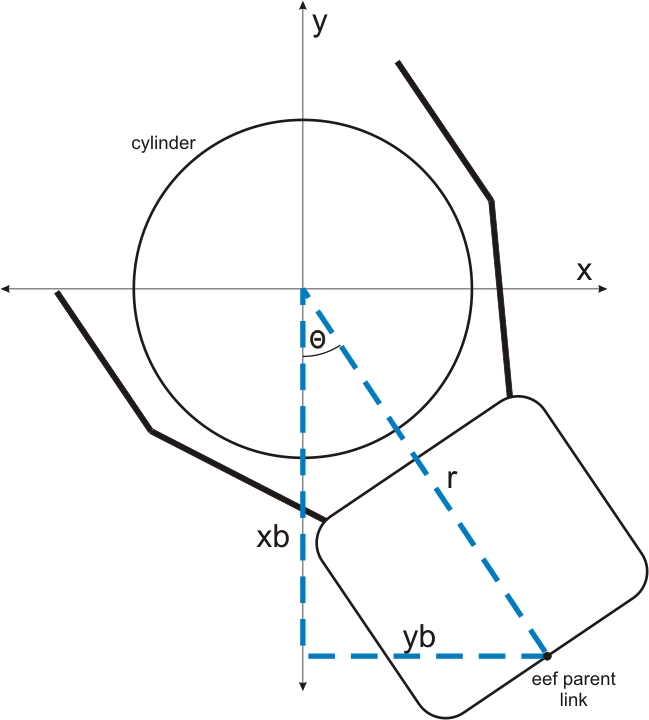
\includegraphics[width=0.4\textwidth]{images/grasps.jpg}
	\caption{Grasp pose determination}
	\label{fig:grasp_pose}
\end{figure}

\paragraph{Grasp quality} This parameter allows to tell the planner, how `good' a specific grasp is, i.e. how likely it is that the grasp can be successfully executed. MoveIt can then favour grasps with higher quality if several valid solutions are found by the planner. As none of the generated grasps should be favoured among the others, all grasps use the quality parameter value $1.0$, which indicates that they are equal in quality.

\paragraph{Allowed touch objects} A list, containing the identifiers of the objects, that are allowed to be touched when using that specific grasp. In the benchmark task, this is only the grasped object.

\subsection{Planning and executing the pickup}

After generating the set of grasps, the pickup operation can be planned. The \emph{PickupAction} server handles planning and optionally the execution of all stages of a pickup operation at once. The request is done, using a \emph{PickupAction} client to send \emph{PickupGoal} messages to the server. The required parameters of the request message are described in the subsequent paragraphs.

\paragraph{\texttt{target\_name}} The name of the object to pick which is the ID that was used when adding the object to the planning scene.
\paragraph{\texttt{group\_name}} The name that identifies the planning group that should be used to perform the pickup, i.e. \path{right_arm}.
\paragraph{\texttt{end\_effector\_name}} The name of an end effector in the specified planning group. This is necessary because it is possible to define planning groups that contain multiple end effectors.
\paragraph{\texttt{possible\_grasps}} The set, containing the previously computed grasps. At least one grasp has to be provided, but the success rate rises when providing multiple grasps.
\paragraph{\texttt{support\_surface\_name}} The name of the link that acts a support surface within the planning scene. This is the link that states the surface mat covering the table (\path{table_surface_link}). 
\paragraph{\texttt{allow\_gripper\_support\_collision}} That parameter specifies, whether collisions between the gripper links and the support surface are allowed, or not.
\paragraph{\texttt{path\_constraints}} It is possible to apply a set of path constraints to the planning request. This could be for example an orientation constraint for the end effector. Path constraints are enforced on each single point of the resulting trajectory which drastically raises the complexity of the planning problem. The sample task does not apply any task constraints.
\paragraph{\texttt{allowed\_planning\_time}} The maximum amount of time, the planner is allowed to find a solution. The sample tasks uses a value of 5 seconds.
\paragraph{\texttt{plan\_only}} Specifies, if resulting trajectories should be immediately executed, or not. This is set to \path{true} to allow a visual validation of the resulting motion plan. \\

On success, the pickup action server returns a motion plan, containing trajectories for all stages of the pickup operation. MoveIt automatically publishes planned trajectories to the \path{move_group/display_planned_path} topic. RViz can be configured to display the trajectories published to that topic. If a visual validation results in a satisfying solution it can be executed on the \path{execute_kinematic_path} service, which is advertised by the \path{move_group} node. The service sends given trajectories to the responsible controller and provides feedback information about the execution status in the service response message. The pickup phase completes after successful execution of all trajectory stages.

%A reusable helper class was created that can be used to simplify all kinds of planning requests. The utility class is called \emph{PlanningHelper} and can be found within the \path{uibk_planning_node} package. A call to the pickup action server is done by using the \path{plan_pick()} method of the helper class. This method takes the a set of possible grasps and the ID of the object to pick as parameters. The outcome is a pointer to an instance of \emph{PlanningResult}, a structure that contains all the necessary information about a planning attempt. Success or failure is indicated by the \path{status} parameter. On success, the parameter \path{trajectory_stages} holds a vector, containing the resulting trajectory stages. The actual planning request is done, using a \emph{PickupAction} client to send \emph{PickupGoal} messages to the pickup server. The message is composed from  the ID of the object to pick, the previously computed grasps, the name of the chosen planning group and the name of the link within the robot model that acts as the support surface. Optional parameters are among others the ID of the planner to use and the maximum allowed planning time. The parameter `plan\_only' within the planning options is set to true to avoid the immediate execution of the planned trajectories. This allows a visual verification of the planning outcome before execution. The resulting robot path is shown in RViz. If the solution is satisfying it can be executed, passing the PlanningResult to the corresponding method of the PlanningHelper class. This method uses the `/execute\_kinematic\_path' service provided by the `move\_group' node. The service sends a given trajectory to the responsible controller and provides feedback information about the execution status. The `PlanningHelper' also takes care to attach the picked object to the gripper after the grasp stage. The pickup phase completes after successful execution of all trajectory stages.


\subsection{Planning and executing the placement}

The placement phase is planned and executed in a similar manner. The cylinder has to be placed on a specific location within the workspace in an upright position - the rotation around the z-axis doesn't matter. Therefore a set of possible place poses is generated in 20 different orientations around the z-axis (Figure \ref{fig:place_stages}a), allowing the planner to choose which one to use. The final approach towards the goal location is specified as \emph{GripperTranslation}. The direction vector points down along the z-axis of the world (Figure \ref{fig:place_stages}b). Desired and minimum distances are set to 20 cm and 10 cm respectively. The same pre-grasp posture configuration is used for the post-place posture. The last required parameter for a place location is the \emph{GripperTranslation} which describes the retreat after releasing the object at the target location. The direction depends on the chosen orientation and points towards the negative z-axis of the gripper reference frame (Figure \ref{fig:place_stages}c). 

\begin{figure}[ht]
	\centering
  	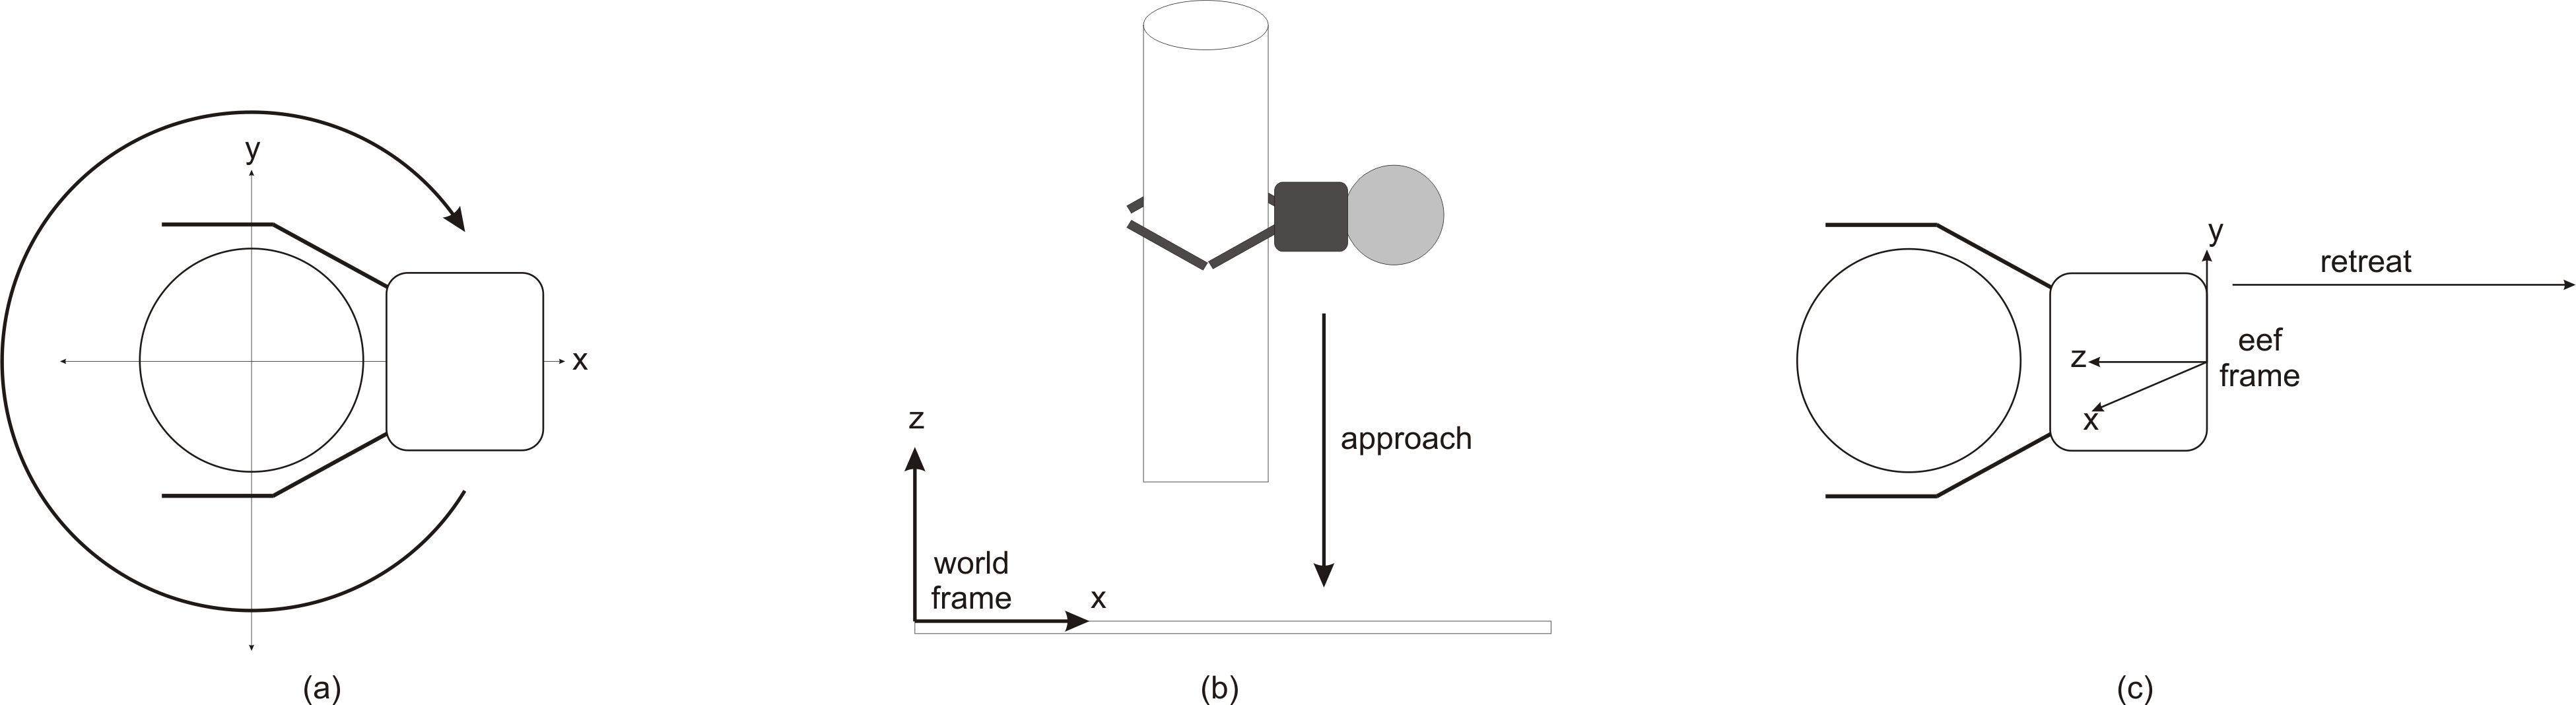
\includegraphics[width=1.0\textwidth]{images/place_a-c.jpg}
	\caption{Place locations, pre-place approach and post-place retreat}
	\label{fig:place_stages}
\end{figure}

The \emph{PlaceAction} server is responsible for planning the whole placement phase. The request utilizes a \emph{PlaceAction} client and \emph{PlaceGoal} messages. The server call is done in the same way as in the pickup phase. The most important parameters are the ID of the object to place, the name of the planning group, the set of possible place locations and the maximum allowed planning time.  On success, again the resulting trajectories are visualized in RViz and can be executed after positive validation. After execution, the task is considered to be completed and the picked object is detached from the gripper and again part of the collision world.


\section{Running the benchmark task}

The benchmark task is designed to run on the simulator and with the real robot as well. It only depends on a running \path{move_group} instance. Therefore it is necessary to start the simulator or real robot and launch the corresponding MoveIt instance as described in Section \ref{sec:launch_moveit}. The benchmark task can then be executed in the desired namespace. This is done by setting the \path{ROS_NAMESPACE} environment variable to either \path{simulation} or \path{real} within the terminal that is used to run the task. The following example runs the benchmark task on the simulator.

\begin{quote}
\begin{verbatim}
export ROS_NAMESPACE=simulation
rosrun uibk_moveit_tests sample_pick_place 
\end{verbatim}
\end{quote}

After creating the environment and adding the objects to the planning scene the pickup phase gets planned. The outcome can be seen in RViz and the program will ask if the resulting trajectory is ok and should be executed. A negative answer will force the program to replan the pickup and ask again, otherwise the trajectory gets executed. After successful execution, the place phase gets planned. The resulting plan is visualized as well and its execution also needs confirmation. The program exits after successful completing the placement phase. Listing \ref{lst:pick_place} shows the main routine of the benchmark task. It was observed that planning sometimes fails due to unknown MoveIt internal issues and subsequent calls with the same parameters are successful. Therefore, the pickup and the place operation are handled within a loop. 

\lstset{style=customc}
\begin{minipage}{\linewidth}
\begin{lstlisting}[caption={Benchmark task main routine}, label=lst:pick_place]
bool start() {
	// create obstacle and object to move...
	createEnvironment();

	bool picked = false;
	while (!picked && ros::ok()) {
		if (!pick(start_pose_, OBJ_ID)) {
			ROS_ERROR_STREAM_NAMED("pick_place", "Pick failed. Retrying.");
			// ensure that object is detached from gripper
			cleanupACO(OBJ_ID);
		} else {
			ROS_INFO_STREAM_NAMED("pick_place",	"Done with pick!");
            picked = true;
		}
	}

	ROS_INFO_STREAM_NAMED("simple_pick_place", "Waiting to put...");
	ros::Duration(5.5).sleep();

	bool placed = false;
	while (!placed && ros::ok()) {
		if (!place(goal_pose_, OBJ_ID)) {
			ROS_ERROR_STREAM_NAMED("pick_place", "Place failed.");
		} else {
			ROS_INFO_STREAM_NAMED("pick_place", "Done with place");
			placed = true;
		}
	}
	return true;
}
\end{lstlisting}
\end{minipage}

\section{Discussion}

This section gives an overview of the most important observations that have been made during the implementation of the sample task:

\begin{itemize}

\item

It is very important to provide some degree of freedom to the planner at various points. This is achieved by providing various grasps and place locations during planning requests. The definitions of gripper translations like pre-grasp approach, post-grasp retreat, pre-place approach and post-place retreat also allow to add additional flexibility by setting the desired and minimum distance values accordingly. Very strictly defined planning requests are very likely to fail whereas requests with a higher degree of flexibility drastically raise the overall success rate.

\item

Working with path constraints drastically drops the success rate because of the high complexity of the planning problem. Enforcing path constraints results in a drastically increased planning time and a large number of necessary IK requests. Therefore no path constraints were used within the sample task. It is possible, that a faster IK solution than the one that is currently utilized could help to solve the problem but that was not tested in this project.

\item

It was observed that sometimes planning requests seem to fail due to some MoveIt-internal issues and not because planning was not possible at all. Therefore it is necessary to repeat failed requests because it is very likely that planning succeeds on subsequent attempts. In the sample task implementation, the planning requests are done within a loop. If a request fails, it gets repeated a couple of times. A successful request breaks the loop and continues the execution flow. This strategy is obviously only feasible in the reference task because its configuration was designed to be plannable and executable.

\item

Resulting trajectories should always be visualized and validated before confirming the execution. This can be done, using RViz and/or the simulator. The calculated motion plans might be valid in terms of the defined goal constraints but sometimes they are overly long and unnatural and therefore unsuitable. Moreover, the planner can only take into account what it knows about the robot's environment. Especially in the robot lab the environment changes frequently when new equipment is mounted in the area around the robot. Therefore the visual validation is particularly important to avoid damages on the robot and its environment.

\end{itemize}


